
%Introdución: composta por Obxectivos Xerais, Relación da Documentación que conforma a Memoria, Descrición do Sistema, Información Adicional de Interese (métodos, técnicas ou arquitecturas utilizadas, xustificación da súa elección, etc.).


This project was made in collaboration with the cybersecurity company Tarlogic SL, even though I am not a member of Tarlogic and have never worked with them in the past. It is key to note my lack of experience in cybersecurity (on a professional level) because is the reason for the bad planning estimations and the limit of the scope. Furthermore in this project there are no absolute constraints or objectives, as it was suggested as a case between investigation (with some coding) and cybersecurity auditing, so the scope can be reduced if the time remaining is too short.

\section{Motivation}

Cybersecurity nowadays is very complex and there are many sub-fields and expert tools and it could be argued that is impossible to guarantee that any system is totally safe. In this project to decide the technologies and tools to use we put ourselves in the shoes of an administrator of an enterprise system that wants to improve the security by detecting intrusions for the servers he works on.
\linej
\linej
Cybersecurity measures can be applied in multiple layers of the system, each with different tools, objectives, advantages and cost. In general the security of a system has the next parts:
\begin{enumerate}
	\item \textbf{Firewall}: Control the inbound/outbound connections, on the \textbf{network layer}. In our case its objective is to reduce the amount of inbound connections, reducing the chance of intrusion.
	\item \textbf{IPS}: Intrusion Prevention System to minimize the chance of intrusions, on the \textbf{network and host layers}. Provides active protection by actions.
	\item \textbf{IDS}: Intrusion Detection System to mitigate the damage of intrusions, on the \textbf{network and host layers}. Provides passive protection by alerts.
\end{enumerate}

\linej
The next table shows a \textbf{simplified} flow on how the information is processed by the security layers and methods. For example an IDS can monitor the network connections, scanning the whole packet (header and payload) and filing a report if needed, but has worse performance than a firewall because they only scan the header of the packet and just opt to reject them\cite{firewall-ipds-ids_comparison}.

\begin{table}[H]
	\centering
	\caption{Simplification of the data flow}
\linej
	\begin{tabular}{|c|c|c|c|}
	\hline
		\textbf{Layer} & Network & \multicolumn{2}{c|}{Network and Host}\\ \hline
		\textbf{Method} & Firewall & IPS & IDS\\ \hline
		\textbf{Measures} & Prevent & Prevent & Mitigate\\ \hline
	\end{tabular}
\end{table}
$\xrightarrow{\makebox[\textwidth]{Direction of the data flow}}$


\linej
\linej
We focus on IDS because we are more interested about host detection. Also IDS is less explored than IPS or Firewall and due to the advance in gathering and processing of data in the last years IDS has become much more viable and reliable.

\linej
\linej
IDSs are different from antivirus or antimalware because the first are systems \textbf{specialized} in detection and the latter usually focus on prevention, however prevention and detection are often meshed together because both are deeply related. There are some cases where a system specialized in detection offers some kind of mitigation functionality or a steam specialized in prevention offers some kind of detection functionality.

\linej
\linej
It is important to note that in cybersecurity the trend is for the attack to be created first and later some kind of measures, not necessarily by the same teams as they usually are specialized in each role. This means that defensive security that requires manual intervention always lags behind.
\linej
Nowadays there are lots of different attacks, so many that their detection could be almost impossible one by one, but most of them can be detected because they share patterns. If we can determine the patterns of an attack and code a way to detect them we can detect the threat. Due to all this some times is easier to detect the attack and take measures after the intrusion has taken place.
\linej
\linej
IDS work by analysing the key information available (programs, logs, network, etc) to determine if there has been an intrusion in the system. The details of the process vary with each IDS but in general they work like an expert system:
\begin{itemize}
	\item The source of the data is the system.
	\item The alerts are set by certain rules when they match.
	\item Rules do not need to throw an alert and there can be dependencies, allowing a stateful approach and complex analysis without false positives (the main annoyance of IDSs).
\end{itemize}

\linej
There are two types of IDS depending of the detection mechanism:
\begin{itemize}
	\item Signature based: The IDS looks for specific data (signature), for example a string. This is often an efficient solution to known attacks, but is fundamentally useless against unknown attacks (attacks without a signature in the IDS database).
	\item Behaviour analysis: After a training period the IDS can detect when an event is rare (by probability) and correlate these suspicious occurrences to an intrusion.
\end{itemize}
In our case we take interest in the signature approach because is much more used and behavior analysis is more fit for network than host.

\linej
\linej
OSSEC is an HIDS (Host-based IDS) solution with detection based on rules and decoders. Both rules and decoders can be defined with numerous options and support dependencies and regular expressions.
\begin{itemize}
	\item The decoders format the data for the rules.
	\item The rules determine there is a threat if the conditions are met.
\end{itemize}
\linej
\textbf{OSSEC} stands for \textbf{O}pen \textbf{S}ource HIDS \textbf{SEC}urity and is interesting for this project because the next qualities\cite{ossec}\cite{wazuh_additional_functionality}:
\begin{itemize}
	\item \textbf{Widely Used}: OSSEC is a growing project, with more than 5,000 downloads per month on average. It is being used by ISPs, universities, governments and even large corporate data centers as their main HIDS solution. In addition to being deployed as an HIDS, it is commonly used strictly as a log analysis tool, monitoring and analyzing firewalls, IDSs, web servers and authentication logs.
	\item \textbf{Scalable}: Because it is an HIDS and it uses \textbf{agents}. Each monitored host can either install the agent or use an agentless agent\cite{agentless}\cite{ossec_agent}. Agentless agents are processes initiated from the OSSEC manager, which gather information from remote systems, and use any RPC method (e.g. ssh, snmp rdp, wmi).
	\item \textbf{Multi-platform}: GNU/Linux, Windows, Mac OS and Solaris. This is important because most professional services are on GNU/Linux or Windows, but it is important to note that rules can only work in one operating system.
	\item \textbf{Free}: OSSEC is a free software and will remain so in the future; you can redistribute it and/or modify it under the terms of the GNU General Public License (version 2) as published by the FSF -- Free Software Foundation.
	\item \textbf{Open source}: The code is open, so you can read, contribute and debug it all you want.
	\item \textbf{Rootkits detection}: This type of malware usually replaces or changes existing operating system components in order to alter the behavior of the system. Rootkits can hide other processes, files or network connections like itself.
	\item \textbf{File integrity monitoring}: To detect access or changes to sensitive data.
\end{itemize}
\linej
There are lots of alternatives to OSSEC for the scenario of a system administrator that wants to reinforce the security of the systems he is responsible for. There are free of charge and paid solutions and they do not need to be pure IDS as often they come in a full approach. For example the next table shows a comparison of the most important ICSs (Industrial Control Systems):
\begin{figure}[H]
  \centering
	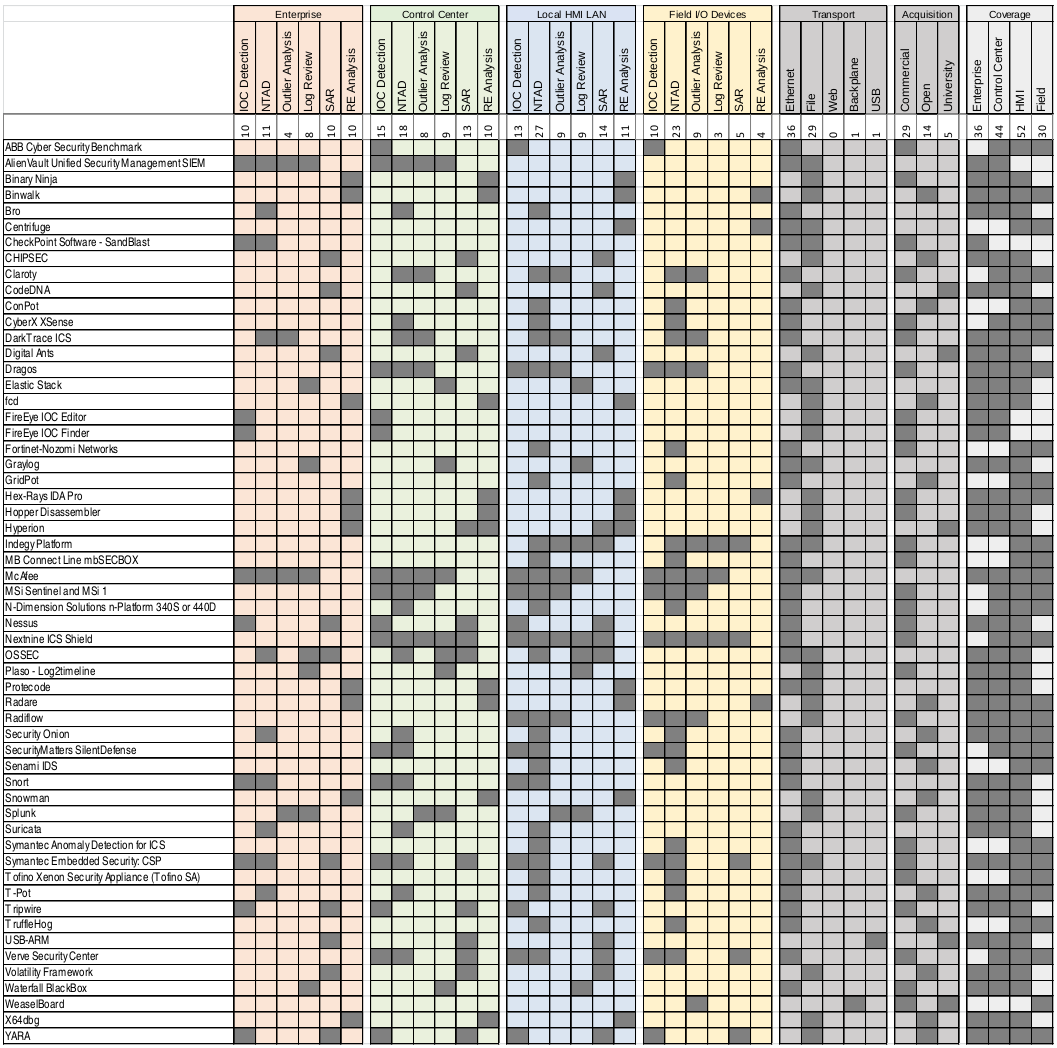
\includegraphics[width=\textwidth]{figuras/comparison_ics.png}
	\caption{Comparison by attributes of the most important ICSs\cite{comparison_ics}}
\end{figure}

\linej
\linej
One of the problems of a comparison in a table like this is that it fails to show how much a tool excels or lacks in the features it shares with others, how easy it is to use and other factors that can decide the right tool. The most relevant alternative technologies to OSSEC for this project are\cite{comparison_tools}:
\begin{itemize}
	\item Bro: Is an open source Network Intrusion Detection System (NIDS), so it does not have any other functionality and supports only Linux, FreeBSD, and Mac OS.
	\item Snort: Is the most popular open source IDS/IPS, but it is only for network and can be very expensive in processing power.
	\item Suricata: Another open source network security monitor with IDS and IPS capabilities and it provides hardware acceleration and multi-threading to improve the scanning speed at the cost of resources.
	\item Sagan: An open source HIDS, but only supports *nix operating systems (Linux, FreeBSD, OpenBSD, etc) and it lacks in features compared to OSSEC.
	\item YARA: Is not an IDS or IPS, it is just a tool that does pattern/string/signature matching, but it excels at it in performance, results and easiness to write the rules. YARA is being used widely in cybersecurity, for example by Avast, Kaspersky Lab, VirusTotal and McAfee Advanced Threat Defense\cite{who_is_using_yara}. We could build a system to use YARA to scan files but always combined with at least another tool, but we prefer to stick to a tested IDS.
\end{itemize}
\linej
In our case most of the attributes in the previous comparison do not matter and we chose OSSEC because the problems found on the alternatives and that OSSEC offers a reliable way to use an already done and thoroughly tested IDS and enhance it to our needs without much work. To even ease more this we will use Wazuh, a fork of OSSEC.





\section{Objectives}
%TODO
The main objective is to improve intrusion detection in IDS. This can be accomplished in several ways:
\begin{itemize}
	\item Adding or changing functionality of an already existing technology.
		\subitem Coding on core or additions.
		\subitem Configuration or input of the program.
	\item Develop a new technology or tools that result in a different detection system.
\end{itemize}

\linej
As mentioned before in this project we will use OSSEC through Wazuh to code rules and decoders, without the need to change any code of the program itself, which means this project can focus directly on detection without the need to create a detection system. Of course if in later stages of the project it would to be found that is convenient to modify the detection system itself it could be considered depending on the importance, the progress and the remaining time of the project.


\section{Structure of this document}
%TODO
This document has TODO chapters:
\begin{itemize}
	\item In \textbf{chapter 1} 
	\item In \textbf{chapter 2} 
	\item In \textbf{chapter 3} 
	\item In \textbf{chapter 4} 
	\item In \textbf{chapter 5} 
	\item In \textbf{chapter 6} 
	\item In \textbf{chapter 7} 
\end{itemize}
